%
% File nodalida2015.tex
%
% Contact beata.megyesi@lingfil.uu.se
%
% Based on the instruction file for EACL 2014
% which in turn was based on the instruction files for previous 
% ACL and EACL conferences.


\documentclass[11pt]{article}
\usepackage[T2A,T1]{fontenc}
\usepackage[utf8]{inputenc}
\usepackage[russian,english]{babel}

\usepackage{times}
\usepackage{latexsym}
\usepackage{fixltx2e} %allows subscripts
\usepackage{tipa} %allows IPA symbols
\usepackage{linguex}
\usepackage{multicol}
%\usepackage[multiple]{footmisc} % separates consecutive footnotes with comma
%\usepackage{mathptmx}
%\usepackage{txfonts}
\usepackage{url}
\usepackage{alltt}
\usepackage{graphicx}
\usepackage[small,bf]{caption}
\special{papersize=210mm,297mm} % to avoid having to use "-t a4" with dvips 
%\setlength\titlebox{6.5cm}  % You can expand the title box if you really have to

\usepackage{nodalida2015}

\usepackage{linguex}
\usepackage{needspace}

\newcommand{\rus}[1]{\foreignlanguage{russian}{#1}}

\newcommand{\ft}[1]{\marginpar{\scriptsize F: #1}} % Fran's comments
\newcommand{\rr}[1]{\marginpar{\scriptsize R: #1}} % Rob's comments

\title{A preliminary constraint grammar for Russian}

\author{Francis M. Tyers \\
  HSL-fakultehta, \\
  UiT Norgga árktalaš universitehta, \\
  N-9018 Romsa \\
  {\tt francis.tyers@uit.no} \\\And
  Robert Reynolds \\
  HSL-fakultehta, \\
  UiT Norgga árktalaš universitehta, \\
  N-9018 Romsa \\
  {\tt robert.reynolds@uit.no} \\}

\date{2015}

\begin{document}
\maketitle
\begin{abstract}
 This paper presents preliminary work on a constraint
 grammar based disambiguator for Russian. Russian is
 a Slavic language with a high degree of both in-category
 and out-category homonymy in the inflectional system.
 The pipeline consists of a finite-state morphological
 analyser and constraint grammar. The constraint 
 grammar is tuned to be high recall (over 0.99) at the expense of 
 low precision.
% \rr{add results to abstract}
\end{abstract}

\section{Introduction}

This paper presents a preliminary constraint grammar for Russian. The main 
objective of the constraint grammar is to produce a high recall grammar to serve
as input into other natural language processing tasks. There are two reasons to
maintain high recall. First, one of the primary applications for this constraint grammar
is computer-assisted language learning. In the domain, erroneous analyses can lead to
significant frustration for learners. Therefore, it is important to limit disambiguation
to cases that can be resolved with high confidence.
Second, it is frequently the case that competing readings can
be distinguished only by considering idiosyncratic collocational information. For such cases, 
we expect that probabilistic approaches are both more effective and simpler to implement.

The paper is laid out as follows: section~\ref{sec:lit} presents a review of 
the literature on Russian language processing; section~\ref{ambiguity} gives
an overview of ambiguity in Russian; section~\ref{sec:pipeline} describes
our analysis pipeline; section~\ref{sec:devel} gives an account of our 
development process; section~\ref{sec:eval} presents an evaluation of the 
system, and sections~\ref{sec:future} and ~\ref{sec:conclusions} present future
work and conclusions.

%Our purposes: Processing stressed wordforms and open-source machine translation

%\cite{Karlsson-90}

% objectives:
%% make a free/open-source morphology for russian based on Z's dictionary that includes stress

\section{Review of literature}
\label{sec:lit}
State-of-the-art morphological analysis in Russian is primarily based on
finite-state technology
\cite{Nozhov-03,Segalovich-03}.\footnote{Machine-learning approaches have also been successfully applied to Russian, most notably by 
\newcite{sharoff08lrec-mocky}.} Almost without exception, all large-scale 
morphological transducers of Russian are based on the
forward-looking \emph{Grammatical Dictionary of Russian} \cite{Zaliznjak-77}.
This dictionary gives fine-grained morphological specifications for more than
100~000 words, including inflectional endings, morphophonemic alternations, 
stress patterns, exceptions, and idiosyncratic collocations.
We developed a morphological transducer based on Zaliznjak's dictionary.\footnote{Our transducer is implemented using a two-level 
morphology \cite{Koskenniemi-84}, and can be compiled using either {\tt xfst}
\cite{Beesley.Karttunen-03} or {\tt hfst} \cite{hfst-11}} This finite-state transducer (FST) generates all possible 
morphosyntactic readings of each wordform, regardless of its frequency or probability. Because Russian is a relatively highly inflected language, broad coverage is important, but widespread homonymy leads to the generation of many spurious readings, as discussed in Section~\ref{ambiguity} below. Because of this, one of the foundational steps in Russian natural language processing is homograph disambiguation.

% FRAN
% different CGs 
% faroese
% estonian

% -- and our Constraint 
%Grammar\footnote{Implemented using vislcg3 constraint grammar parser
%(\url{http://beta.visl.sdu.dk/cg3.html}).}
%\cite{Karlsson-90,Karlsson.Voutilainen.ea-95} then removes
%some readings based on syntactic context.

%\cite{trosterud2009}

% CGs for Slavic langs

% The preliminary tagging performance is P:,96.1%, R:,99.8% for POS tagging and P:,88.2%, R:,98.1% for complete morphosyntactic tagging.
% \cite{peradin12} 

\section{Ambiguity in Russian} \label{ambiguity}

We identify three different types of morphosyntactic ambiguity: 
intraparadigmatic, morphosyntactically incongruent, and morphosyntactically 
congruent. The following examples make use of word stress ambiguity to illustrate 
each kind of ambiguity.\footnote{Written standard Russian does not typically
indicate stress position, but knowing stress position is essential for pronunciation. 
A recent study by \newcite{reynolds.tyers-15} found that about 7.5\% of 
morphosyntactic ambiguity in a corpus of Russian resulted in stress position 
ambiguity.} \emph{Intraparadigmatic} ambiguity refers to homographic 
wordforms belonging to the same lexeme, as shown in \ref{ex:intrahom}. 

\needspace{4\baselineskip} % keeps example all together (no orphan line) 
\ex. Intraparadigmatic homographs \label{ex:intrahom}
\a. \rus{т\'{е}ла} \emph{t\'{e}la} `body.\textsubscript{SG-GEN}' 
    \label{ex:bodySGGEN}
\b. \rus{тел\'{а}} \emph{tel\'{a}} `body.\textsubscript{PL-NOM}' 
    \label{ex:bodyPLNOM}

The remaining two types of ambiguity occur between lexemes. 
\emph{Morphosyntactically incongruent} ambiguity occurs between homographs that 
belong to separate lexemes, and whose morphosyntactic values are different, as 
shown in \ref{ex:MSincongruent}.

\needspace{4\baselineskip} % keeps example all together (no orphan line) 
\ex. Morphosyntactically incongruent homographs \label{ex:MSincongruent}
\a. \rus{н\'{а}шей} \emph{nášej} `our.\textsubscript{F-SG-GEN/DAT/LOC...}'\\
    \rus{наш\'{е}й} \emph{našéj} `sew on.\textsubscript{IMP-2SG}'
\b. \rus{дор\'{о}га} \emph{doróga} `road.\textsubscript{N-F-SG-NOM}'\\
    \rus{дорог\'{а}} \emph{dorogá} `dear.\textsubscript{ADJ-F-SG-PRED}'

\emph{Morphosyntactically congruent} ambiguity occurs between homographs 
that belong to separate lexemes, and whose morphosyntactic values are identical, 
as shown in \ref{ex:MScongruent}.

\needspace{6\baselineskip} % keeps example all together (no orphan line) 
\ex. Morphosyntactically congruent homographs \label{ex:MScongruent}
\a. \rus{з\'{a}мок} \emph{z\'{a}mok} `castle.\textsubscript{SG-NOM}'\\
	\rus{зам\'{о}к} \emph{zam\'{o}k} `lock.\textsubscript{SG-NOM}'
\b. \rus{з\'{a}мков} \emph{z\'{a}mkov} `castle.\textsubscript{PL-GEN}'\\
	\rus{замк\'{о}в} \emph{zamk\'{o}v} `lock.\textsubscript{PL-GEN}'\\
    etc.

Table \ref{table:ambiguity} shows the prevalence of each kind of 
ambiguity. The first column shows the proportion 
of all tokens in a corpus that have each kind of ambiguity. The second column 
shows what proportion of ambiguous tokens exhibit each kind of ambiguity.
Note that these proportions do not sum to 100\%, since a given token may 
exhibit more than one kind of ambiguity. For example, the wordform 
\emph{zamkov} has the readings given in \ref{ex:zamkov}.

\ex. \label{ex:zamkov}
	 \a. \rus{замок}$^1$+N+Msc+Inan+Pl+Gen \label{ex:zamkovA}
	 \b. \rus{замок}$^2$+N+Msc+Inan+Pl+Gen \label{ex:zamkovB}
	 \c. \rus{замковый}+A+Msc+Sg+Pred      \label{ex:zamkovC}

The ambiguity between \ref{ex:zamkovA} and \ref{ex:zamkovB} is morphosyntactically congruent, and
the ambiguity between \ref{ex:zamkovA}/\ref{ex:zamkovB} and \ref{ex:zamkovC} is
morphosyntactically incongruent, so this wordform would be counted for both categories in
Table~\ref{table:ambiguity}.

Table~\ref{table:ambiguity} shows that most morphosyntactic ambiguity in 
unrestricted Russian text is rooted in intraparadigmatic and morphosyntactically 
incongruent ambiguity. Detailed part-of-speech tagging with morphosyntactic 
analysis can help disambiguate these forms. On the other hand, morphosyntactically congruent
ambiguity represents only a very small percentage of ambiguous wordforms, and instead 
of detailed part-of-speech tagging, it can be resolved by means of word sense disambiguation.
Because of this difference, we leave morphosyntactically congruent ambiguity to future work.

\begin{table}[ht]
  \centering
  \begin{tabular}{l|rr}
    \hline
    \textbf{Type}  & \textbf{all tokens} & \textbf{ambig. tokens} \\
    \hline
    Intraparadigm. & 59.0\%                   & 90.9\%   \\
    Incongruent    & 27.7\%                   & 42.7\%   \\ 
    Congruent      & 1.2\%                   & 1.8\%    \\ 
    \hline
  \end{tabular}
  \caption{Frequency of different types of morphosyntactic ambiguity in unrestricted text}
  \label{table:ambiguity}
\end{table}

% we should perhaps mention something about systematic ambiguities and tagging guidelines,
% and how we deal with stuffs
% e.g. adj/participle
%      det/pron
%      acc2/nom
%      lexicalised passive / pass

% perhaps mention where our annotation guidelines are (do we mention stuff like один)?

\section{Pipeline}
\label{sec:pipeline}
% FRAN

\subsection{Morphological analyser}
\label{sec:morph}
%ROB

The morphological transducer used in this study is 
primarily based on Zaliznjak's \emph{Grammatical dictionary of Russian}, 
including the 2001 version's appendix of proper nouns. It also includes neologisms
from Grishina and Lyashevskaya's \emph{Grammatical dictionary of new Russian words},
which is intended to be a supplement to Zaliznjak's dictionary with words found in
the Russian National Corpus.\footnote{\url{http://dict.ruslang.ru/gram.php}} 
Example~\ref{ex:FSToutput} gives some examples of the FST's output.

\ex. \label{ex:FSToutput} 
	\a. \rus{новый}\texttt{{\small <adj><m><nn><sg><nom>}}\\
	    `new'
	\b. \rus{автомат}\texttt{{\small <n><m><nn><sg><nom>}}\\
	    `automaton, sub-machine gun'
%	\c. 
% det/prn (e.g. pos... их, я, мой)
% 'over'generation (e.g. all dets get all gen/nbr/case combinations)
%^^^
%ROB

\subsection{Disambiguation rules}
%FRAN

The constraint grammar is composed of 299 rules which are divided into four
categories: Safe, Safe heuristic, Heuristic, and Syntax labeling. The distribution
of rules is shown in Table~\ref{tab:ruleDist}.

\begin{table}
  \centering
  \begin{tabular}{lrrr}
    \hline
                     & {\sc select} & {\sc remove} & {\sc map} \\
    \hline
    Safe             &   16         &   34         &  -- \\
    Safe heuristic   &   89         &   76         &  -- \\
    Heuristic        &   26         &   52         &  -- \\
    Syntax labelling & --           & --           & 6 \\ 
    \hline
  \end{tabular}
  \caption{The 299 rules in the grammar are separated into four sections depending
      on rule reliability. }
  \label{tab:ruleDist}
\end{table}

The philosophy is that Safe rules should represent real constraints in
the language. Examples might be that a preposition cannot directly precede a finite verb
or that prepositional case requires a preceding preposition. 

% Examples where this might go wrong:
% This rule can fail in dialogs where the preposition is explicit in the previous turn.

Safe heuristic rules should deal with highly frequent tendencies in the language.
For example remove a genitive at the beginning of a sentence if it is capitalised
and there is no verb governing the genitive found to the right and there is also no
negated verb to the right. This rule relies on the fact that if the genitive is in first 
position in the sentence it cannot modify anything before, and no preposition 
can be governing it. This kind of rule often relies on completeness of sets, 
in this case the set of verbs that can take a genitive complement.

%It also relies on accurate delimitation of sentence
%boundaries, including rules for dealing with \ldots ellipsis.

% Examples where this might go wrong:
% Russian has relatively free word order. Technically there is no grammatical limitation
% from having a genitive noun modifying a noun elsewhere in the sentence.

Heuristic rules are those which we do not consider linguistic constraints, but express
preferences, often dealing with overgeneration or overspecification in the morphological
transducer. For example, remove the verbal adverb reading of \rus{такая}, which could be 
the feminine singular nominative of \rus{такой} `such' or the verbal adverb 
of \rus{такать} `say \emph{well}\ldots'.

% Examples where this might go wrong:
% Anywhere that a verbal adverb is possible, especially if there are no feminine nominals
% in the sentence.

Given a large hand-annotated corpus we believe that most of the heuristic rules would be 
better replaced with information learnt from the corpus through stochastic methods. 



\section{Development process}
\label{sec:devel}
%FRAN

A common approach taken when writing constraint grammar rules is to 
apply the existing rule set to a new text, write new rules to deal with the 
ambiguities, then apply the rules to a hand-annotated corpus to see
how often the rule disambiguated correctly \cite{voutilainen99}.

Due to the lack of a hand-annotated corpus compatible with our morphological
analyser, we adopted a slightly modified technique. We picked a random text
from the Russian Wikipedia,\footnote{The Russian Wikipedia was chosen as a testing corpus
  as it is the largest, freely licensed corpus of Russian available on the internet. It is 
  not representative of Russian texts as a whole.}
ran it through the morphological analyser, wrote
%\rr{R1: Is ru-wikipedia representative of Russian texts on the whole?}
rules, and then ran the rules on the whole Wikipedia corpus. For each rule,
we collected around 100 example applications and checked them. If a rule
selected the appropriate reading in all cases, we included it in the \emph{safe}
rule set, if it removed an appropriate reading in less then three cases, 
then we included it in the \emph{safe heuristic} rule set. Otherwise we either
discarded the rule or included it in the heuristic rule set.

\begin{figure*}
\centering
\begin{multicols}{2}
\noindent
\begin{alltt}
{\small

"<\rus{В}>"
    "\rus{в}" pr

"<\rus{ноябре}>"
    "\rus{ноябрь}" n m nn sg prp

"<1994>"
    "1994" num

"<\rus{года}>"
    "\rus{год}" n m nn sg gen SELECT:r462
;   "\rus{год}" n m nn pl nom fac SELECT:r462

"<\rus{в}>"
    "\rus{в}" pr

"<\rus{Танзании}>"
    "\rus{Танзания}" np al f nn pl acc
    "\rus{Танзания}" np al f nn sg prp
;   "\rus{Танзания}" np al f nn pl nom REMOVE:r424
;   "\rus{Танзания}" np al f nn sg dat REMOVE:r433
;   "\rus{Танзания}" np al f nn sg gen REMOVE:r433

"<\rus{начал}>"
    "\rus{начало}" n nt nn pl gen
    "\rus{начать}" vblex perf tv past m sg
;   "\rus{начать}" vblex perf iv past m sg REMOVE:r769

"<\rus{работу}>"
    "\rus{работа}" n f nn sg acc
    
"<\rus{Международный}>"
    "\rus{международный}" adj m an sg nom
    "\rus{международный}" adj m nn sg acc

"<\rus{трибунал}>"
    "\rus{трибунал}" n m nn sg acc
    "\rus{трибунал}" n m nn sg nom

"<\rus{по}>"
    "\rus{по}" pr

"<\rus{Руанде}>"
    "\rus{Руанда}" np al f nn sg prp
    "\rus{Руанда}" np al f nn sg dat
"<.>"
    "." sent
}
\end{alltt}
\end{multicols}
  \caption{Example output from the morphological analyser and constraint grammar for the sentence \rus{В ноябре 1994 
           года в Танзании начал работу Международный трибунал по Руанде.} ``The work of the International Tribunal 
           for Rwanda started in Tanzania in November 1994.'' The input ambiguity is 1.76 readings per word and 
           the output ambiguity is 1.38 readings per word. Recall is 1.0 and precision is 0.72. Figure~\ref{fig:rules} 
           shows the rules that fired for this example sentence.} 
  \label{fig:output}
\end{figure*}

\begin{figure*}

\begin{alltt}
{\small
### Safe

SELECT:r462 Gen IF (0 Year) (-1 Num LINK -1 Months LINK -1 Pr/V);
  # Select genitive reading of `\rus{года}' if there is a numeral immediately
  # to the left, before that there is a month and before that there is 
  # the preposition `\rus{в}'.

REMOVE:r424 Nom IF (-1C Pr) ;
  # Remove nominative case if there is a word which can only be a 
  # preposition immediately to the left.

REMOVE:r433 NGDAIP - Acc - Prp - Loc IF 
                (-1C* Pr/V OR Pr/Na
                  BARRIER (*) - Adv - Comp - DetIndecl - ModAcc - ModPrp);
  # Remove all cases apart from accusative, preposition and locative
  # if `\rus{в}' or `\rus{на}' are found to the left and are unambiguous. The barrier
  # is anything that cannot be found inside a noun phrase.

### Safe heuristic

REMOVE:r769 IV IF (0 TV OR IV) (1C Acc) (NOT 1 AccAdv);
  # Remove an intransitive reading of a verb if the next word can only
  # be accusative and is not in the set of nouns which can be used 
  # adverbially in accusative.
}
\end{alltt}
  \caption{Some example rules from the grammar.}
  \label{fig:rules}
\end{figure*}

\section{Evaluation}
\label{sec:eval}

\subsection{Corpus}
In order to evaluate the grammar we hand-annotated 10,150 words of Russian text
from Wikipedia articles, public domain literature and freely-available news sources. The
annotated texts are available online under the {\sc cc-by-sa} licence.\footnote{\url{https://svn.code.sf.net/p/apertium/svn/languages/apertium-rus/texts/}}
%\rr{is this a good url? Do we need to put a COPYING file in that folder?}

Hand-annotation proceeded as follows: The text was first morphologically analysed, 
and then an annotator read through the output of the morphological analyser, commenting
out the readings which were not appropriate in context. This annotated text was then checked
by a second annotator.

We chose to annotate our own texts as opposed to using a well-known hand-annotated corpus
such as the Russian National Corpus (RNC) for two main reasons: the first was that the 
RNC is not freely available; the second was that the standards for tokenisation, part-of-speech
and morphological description are different from our morphological analyser.

Table~\ref{table:results} gives a quantitative evaluation of the performance of our CG on the test corpus.

\subsection{Qualitative evaluation}
%FRAN

In this section, we give a qualitative evaluation of errors made by the CG.

\begin{table*}
  \centering
  \begin{tabular}{|l|r|r|r|r|r|}
    \hline
    \textbf{Domain} & \textbf{Tokens} & \textbf{Precision} & \textbf{Recall} & \textbf{F-score} & \textbf{Ambig. solved} \\
    \hline
    Wikipedia       & 7,857      & 0.506        & 0.996    & 0.671 & 44.92\%  \\
    Literature      & 1,652      & 0.473        & 0.984    & 0.638 & 42.95\%  \\
    News            & 642        & 0.471        & 0.990    & 0.638 & 41.60\%  \\
    \hline
    \textbf{Average}& 10,150     & 0.498        &  0.994   & 0.663 & 44.39\% \\
    \hline
  \end{tabular}
  \caption{Results for the test corpora.}
  \label{table:results}
\end{table*}


%\begin{table}
%  \centering
%  \begin{tabular}{|l|r|r|}
%    
%    \hline
%    Error in original        &   & 2  \\
%    Missing lexeme           &   & 8  \\   % безбалластный, FALSENEG: Кий<np><ant><m><sg><ins> ['кий<n><m><nn><sg><ins>']
%    Partial lexeme           &   & 2  \\   % франко-норманнское, рельс
%    Missing analysis         &   &    \\   % 
%    Equally valid analysis   &   &    \\   % большой<adj><comp><pred> ['больше<adv>'] (?)
%    Correct reading removed  &   & 34 \\   % 
%    \hline
%                             &   & 46 \\
%    \hline
%  \end{tabular}
%  \caption{Error analysis of false negatives}
%\end{table}

% unknown words from test corpus, categorisation

% rule error analysis

\begin{description}
  \item[ Bad linguistics:] In some cases a rule did not take into account grammatical possibilities 
    in the language. e.g. Two simple rules such as 
    \begin{itemize}
      \item \texttt{REMOVE Det IF (0 Det OR Pron) (1C Ne) ;}
      \item \texttt{REMOVE Det IF (0 Det OR Pron) (1 Cm LINK 1 CC OR CS) ;}
    \end{itemize}
    did not take into account the possibility of having a postposed determiner as in
    \begin{itemize}
      \item \ldots \rus{а может быть и раньше, и факт этот не раз поражал меня} \ldots
      \item \ldots and maybe even earlier, and fact \textbf{this} not once surprised me \ldots
    \end{itemize}
    or a interposed parenthetical as in
    \begin{itemize}
      \item \rus{Но какие, однако же, два разные создания, точно обе с двух разных планет!}
      \item But what, \textbf{exactly} , two different creatures, just both from two different planets!
    \end{itemize}
  \item[ Bad rule:] In some cases a rule was simply incorrectly specified. For example, the 
    following rule was designed to solve the ambiguity between short-form neuter adjectives and 
    adverbs
   \begin{itemize}
     \item \texttt{REMOVE A + Short IF (-1C Fin OR Adv OR A) (0C Short OR Adv) ;}
   \end{itemize}
   However there is no reason why we should prefer an adverb over an adjective after an adverb, 
   \begin{itemize}
     \item \ldots \rus{потому что совсем неприятно проснуться в гробу под землею.}
     \item \ldots because [it is] really \textbf{unpleasant} to wake up in a coffin under the ground.
   \end{itemize}
  \item[ Incomplete barrier:]  Some rules suffered from incomplete barriers, which is something that would
     benefit from a more systematic treatment.
   \begin{itemize} 
     \item \texttt{REMOVE NGDAIP - Acc - Prp - Loc IF (-1C* Pr/V OR Pr/Na BARRIER (*) - Adv - Comp - DetIndecl - ModAcc - ModPrp) ;}
   \end{itemize}
   here the rule removes the nominative reading of the adjective to leave the accusative reading because the preposition \rus{в} `in'
   is found preceeding. 
   \begin{itemize}
     \item \rus{В 1960-х электрифицированные высокоскоростные железные дороги появились в Японии и некоторых других странах.}
     \item In the 1960's \textbf{electrified} high-speed railways appeared in Japan and some other countries.
   \end{itemize} 
  \item[ Incomplete set:] In some cases the rule was a good generalisation, but made use of a set
    which was incomplete. For example:
   \begin{itemize}
     \item \texttt{REMOVE Dat IF (NOT 0 Prn/Sebe) (NOT 0 Anim OR Cog OR Ant) (NOT 0 Pron) (NOT 1* V/Dat) (NOT -1* V/Dat) (NOT -1* Prep/Dat) (NOT -1C A + Dat) ;}
   \end{itemize} 
   the set \texttt{V/Dat} does not contain the verb \rus{противопоставлять} `opposed to' which takes 
   a dative argument.
   \begin{itemize}
     \item \rus{В связи с этим ортодоксальности стали противопоставлять ересь.}
     \item In connection with this \textbf{orthodoxy} was opposed to heresy. 
   \end{itemize}
  \item[ Rule interaction:] The strong accusative rule below causes incorrect behaviour in the rule to remove transitivity readings
  \begin{itemize}
     \item \texttt{REMOVE TV - Pass IF (NOT 1* Acc) (NOT -1* Acc) ;}
     \item \texttt{REMOVE Acc IF (-1C Fin + IV) (NOT 0 AccAdv) ;}
  \end{itemize}
  Consider the following example where \rus{может} `can' is tagged as intransitive, the second rule fires removing 
  the accusative reading of \rus{его} `him', and thus given the lack of accusative reading, \rus{найти} `find'
  is disambiguated as intransitive instead of transitive.
  \begin{itemize}
    \item \rus{Она смотрит везде, но не может его найти.}
    \item She looks around, but she cannot \textbf{find him}.
  \end{itemize}
  \item[ Difficult linguistics:] Dealing with participles with arguments is challenging in the case that the arguments 
    of the participle share the same government as the main verb.
  \begin{itemize}
    \item \texttt{REMOVE IV IF (0 TV OR IV) (1C Acc) (NOT 1 AccAdv) ;}
  \end{itemize}
    Here \rus{Ваню и Машу} `Vanja and Maša' are the object of \rus{видит} `sees' and not \rus{играющих} `playing', although
    both verbs can take accusative object.
  \begin{itemize}
    \item \rus{Их мама внутри дома с кошкой, она смотрит в окно и видит играющих Ваню и Машу.}
    \item Their mother is inside the house with the cat, she looks through the window and sees Vanja and Maša \textbf{playing}.
  \end{itemize}
    This kind of error would ideally be resolved with semantic knowledge. 
\end{description}

%% safe:

% <REMOVE:382>  0       29      0       1
% REMOVE Det IF (1 EOS) ;
% Но, разумеется, никогда нам не исчерпать всего явления, не добраться до конца и начала его.
%+ postposed determiner (or pronoun?)

% <REMOVE:492>  0       12      0       1
% REMOVE Det IF (0 Det OR Pron) (1C Ne) ;
% Это я знал еще с 46-го года, когда начал писать, а может быть и раньше, - и факт этот не раз поражал меня и ставил меня в недоумение о полезности искусства при таком видимом его бессилии.
%+ postposed determiner (факт этот)

% <REMOVE:414>	0	0	0	1
% REMOVE A + Short IF (-1C Fin OR Adv OR A) (0C Short OR Adv) ;
% А если удастся, то я прошу только, чтоб схоронили меня, вполне убедясь, что я мертвая, потому что совсем неприятно проснуться в гробу под землею.
%+ bad rule. adverb (maybe adj too) does not make sense here 

% <REMOVE:433>	0	992	0	1
% REMOVE NGDAIP - Acc - Prp - Loc IF (-1C* Pr/V OR Pr/Na BARRIER (*) - Adv - Comp - DetIndecl - ModAcc - ModPrp) ;
% В 1960-х электрифицированные высокоскоростные железные дороги появились в Японии и некоторых других странах.
%+ incomplete barrier (ordinal in another case)

% <REMOVE:494>	0	60	0	1
% REMOVE Det IF (0 Det OR Pron) (1 Cm LINK 1 CC OR CS) ;
% Но какие, однако же, два разные создания, точно обе с двух разных планет!
%+ parentheticals

%% safe-heuristic:

% <SELECT:718>  0       18      0       1
% SELECT A + $$NGDAIP IF (1C* N + $$NGDAIP BARRIER Punct OR Pr OR Lparen OR NGDAIP - $$NGDAIP LINK -1C* A + $$NGDAIP BARRIER Punct OR Pr OR Lparen OR NGDAIP - $$NGDAIP);
% Движущей силой в поездах являются локомотивы, использующие электричество или производящие собственную мощность, обычно дизельными двигателями.
%+ missing unification on number, rule too loose.

% <REMOVE:769>  0       57      0       1
% REMOVE IV IF (0 TV OR IV) (1C Acc) (NOT 1 AccAdv) ;
% Их мама внутри дома с кошкой, она смотрит в окно и видит играющих Ваню и Машу.
%+ participle is intransitive, because it is modifying Vanju and Mašu, but they are object of видит so look like object of играющих. both syntactically valid, but semantics would tell you that you can't play people.

% <SELECT:692>	0	10	0	2
% SELECT Pron IF (0C Prp) (0 Pron OR Det) (NOT 0 Num) (NOT 1* Prp BARRIER (*) - Adv - DetIndecl) ;
% Наземные цели (танки, бронетранспортёры), характерные для штурмовиков и ударных вертолётов, имеют, в большинстве своём, значительно более тяжёлое и прочное бронирование, чем авиационные, что определяет использование бронебойных снарядов.
%+ postposed determiner своём

% <SELECT:864>	0	13	0	1
% SELECT Nom IF (0C Nom OR Acc) (-1C* Nom BARRIER NGDAIP - Nom - Acc LINK -1C* IV BARRIER NGDAIP - Nom OR TV OR CLB OR Pr) ;
% Если самоубийство не удастся, то пусть соберутся все отпраздновать мое воскресение из мертвых бокалами Клика.
% [ only IV ] (anything not nom) [ only nom ] (any case but nom/acc) [nom or acc]
%+ bad rule

% <REMOVE:784>	0	67	0	2
% REMOVE Acc IF (-1C Fin + IV) (NOT 0 AccAdv) ;
% Я именно заметил ему перед этим, что я, чуть не сорок лет знающий "Горе от ума", только в этом году понял как следует один из самых ярких типов этой комедии, Молчалина, и понял именно, когда он же, то есть этот самый писатель, с которым я говорил, разъяснил мне Молчалина, вдруг выведя его в одном из своих сатирических очерков.
%+ parenthetical (как следует)
%! Было установлено, что после того, как 6 апреля 1994 года в авиакатастрофе погиб президент Хабиаримана, Багосора полностью захватил контроль над политической и военной ситуацией в стране, следовательно несёт ответственность за произошедшие затем события .
%! нести = TV here, but IV ?


% <REMOVE:656>	0	16	0	3
% REMOVE TV - Pass IF (NOT 1* Acc) (NOT -1* Acc) ;
% Она ничего не видит, она считает.
% Люди никогда не получают ответа, когда говорят с собаками!
% Она смотрит везде, но не может его найти.
%+ genitive object

%      REMOVE Acc IF (-1C Fin + IV) (NOT 0 AccAdv) ;
%      bad interaction with auxiliary verb rule, we remove the acc reading on его

%% heuristic:

% <REMOVE:917>	0	533	0	2
% REMOVE Dat IF (NOT 0 Prn/Sebe) (NOT 0 Anim OR Cog OR Ant) (NOT 0 Pron) (NOT 1* V/Dat) (NOT -1* V/Dat) (NOT -1* Prep/Dat) (NOT -1C A + Dat) ;
% В связи с этим ортодоксальности стали противопоставлять ересь 
%+ incomplete set (e.g. стали should appear in V/Dat)
% В противоположность «юбилейной концепции» часть историков и археологов считает, как и прежде, что образование Киева как города проходило в VIII—X веках.
%+ противоположность takes dative (против-) 

% <REMOVE:954>	0	272	0	7
% REMOVE Adv/I IF (NOT -1* Adv/Ješë OR Jest OR Rel OR No BARRIER (*) - Adv) (NOT -1* CC BARRIER (*) - Adv) ;
% А знаете ли вы, - вдруг сказал мне мой собеседник, видимо давно уже и глубоко пораженный своей идеей, - знаете ли, что, что бы вы ни написали, что бы ни вывели, что бы ни отметили в художественном произведении, - никогда вы не сравняетесь с действительностью.
% Действительность тотчас же представит вам в этом же роде такой фазис какой вы и еще и не предлагали и превышающий все, что могло создать ваше собственное наблюдение и воображение!
% Действительность тотчас же представит вам в этом же роде такой фазис какой вы и еще и не предлагали и превышающий все, что могло создать ваше собственное наблюдение и воображение!
% Это я знал еще с 46-го года, когда начал писать, а может быть и раньше, - и факт этот не раз поражал меня и ставил меня в недоумение о полезности искусства при таком видимом его бессилии.
% Но ведь в том-то и весь вопрос: чей глаз и кто в силах? 
% Вот эта-то смерть и напомнила мне о сообщенном мне еще летом самоубийстве дочери эмигранта.
% Зачастую и после убийств над телами жертв совершали издевательства — разрубали их на куски и т. д. 
%+ this is a complete mess, in certain genres, и is much more frequent as an adverb
% probably needs collocation info

% <SELECT:1065>	0	4	0	1
% SELECT $$NGDAIP IF (0 N + $$NGDAIP) (1 @CNP LINK 1 N + $$NGDAIP) ;
% Однако после войны в Афинах, как и в Греции в целом, начался период ускоренного развития, который длился до 1980-х, когда впервые дали о себе знать проблема перенаселения столицы и проблема транспорта.
%+ doesn't take into account genitive modifiers

% <SELECT:1071>	0	37	0	1
% SELECT $$NGDAIP IF (0 N + $$NGDAIP) (-1 @CNP LINK -1 N + $$NGDAIP) ;
% Образ триединого бога есть сферическая поверхность, а именно: бог-отец в центре, бог-сын — на поверхности и святой дух — в симметричном отношении между центром и описанной вокруг него сферической поверхностью.
%+ @CNP should be @CVP because of the тире

% <SELECT:1013>	0	4	0	1
% SELECT Sg IF (0 Prop) (0 Gen) (-1 N) (1 EOS) (NOT -1* Fin + Pl) ;
% Старое здание Афинского университета, расположенное на проспекте Панепистимиу, является одним из самых стильных в городе, наряду с Национальной библиотекой и Академией Афин.
%+ massive hack, not linguistically motivated
%+ could be improved by only applying to ant/pat


\subsection{Task-based evaluation}
% ROB accent placement task

The constraint grammar described in this paper has been applied to the task of automatic
word stress placement \cite{reynolds.tyers-15}. This task is especially relevant for 
Russian language learners, because vowels are pronounced differently depending on their position 
relative to stress position. For example, the word \emph{molokó} `milk' is pronounced 
/\textipa{m@l2kO}/, where each instance of the letter \emph{o} corresponds to a different vowel sound. 
Russian has complicated patterns of shifting stress, which are difficult for learners to master.
Almost 99\% of wordforms with ambiguous stress position can be disambiguated morphosyntactically,
so a constraint grammar can potentially resolve most stress ambiguity indirectly. The results of 
\newcite{reynolds.tyers-15} show that our constraint grammar overcomes about 42\% of the ambiguity 
relevant to stress ambiguity in unrestricted text.

\subsection{Combining with a statistical tagger}

Given that just over half of all ambiguity remains after running our preliminary constraint
grammar and that for many applications unambiguous output is necessary, we decided to 
experiment with combining the constraint grammar with a statistical tagger to resolve remaining
ambiguity. Similar approaches have been taken by previous researchers with Basque \cite{ezeiza.ea-98}, 
Czech \cite{hajic.ea-01,hajic.ea-07}, Norwegian \cite{johannessen.ea-11,johannessen.ea-12}, 
Spanish \cite{hulden12}, and Turkish \cite{oflazer.tur-96}. 

We follow the voting method described by \newcite{hulden12}. We used the freely available
\texttt{hunpos} part-of-speech tagger \cite{halacsy07}. We performed 10-fold
cross validation using our evaluation corpus, taking 10\% for testing and 90\% for training, and
experimented with three configurations:

\begin{itemize}
  \item \texttt{HMM}: the \texttt{hunpos} part-of-speech tagger with its default options
  \item \texttt{HMM+Morph}: as with \texttt{HMM} but incorporating the output of our 
    morphological analyser (see section~\ref{sec:morph}) as a full form lexicon.
  \item \texttt{HMM+Morph+CG}: we submitted the output from \texttt{HMM+Morph} and the 
    constraint grammar to a voting procedure, whereby if the constraint grammar left
    one valid reading, we chose that, otherwise if the constraint grammar left a word
    with more than one reading, we chose the result from the \texttt{HMM+Morph} tagger.
\end{itemize}

As can be seen from Figure~\ref{fig:curve}, incorporating the constraint grammar 
improves the performance of the HMM tagger, an improvement of nearly 5\% in accuracy,
similar to that reported by \newcite{hulden12} for the same amount of training data. 
In Figure~\ref{fig:curve}, it appears that the HMM alone is much more dependent on 
training corpus size than the voting setup, which improves very little between a training
corpus size of 5,000 and 9,000.

Our constraint grammar also has a much lower precision as a result of the ambiguity remaining
in the output. Similarly, the final accuracy is below the state of the art for Russian. For instance, 
\newcite{sharoff08lrec-mocky} report a maximum accuracy of 95.28\% using the TnT tagger.
Note, however, that this model was trained on a much larger corpus -- over five million
tokens -- which is not freely available.

\begin{figure*}
  \centering
  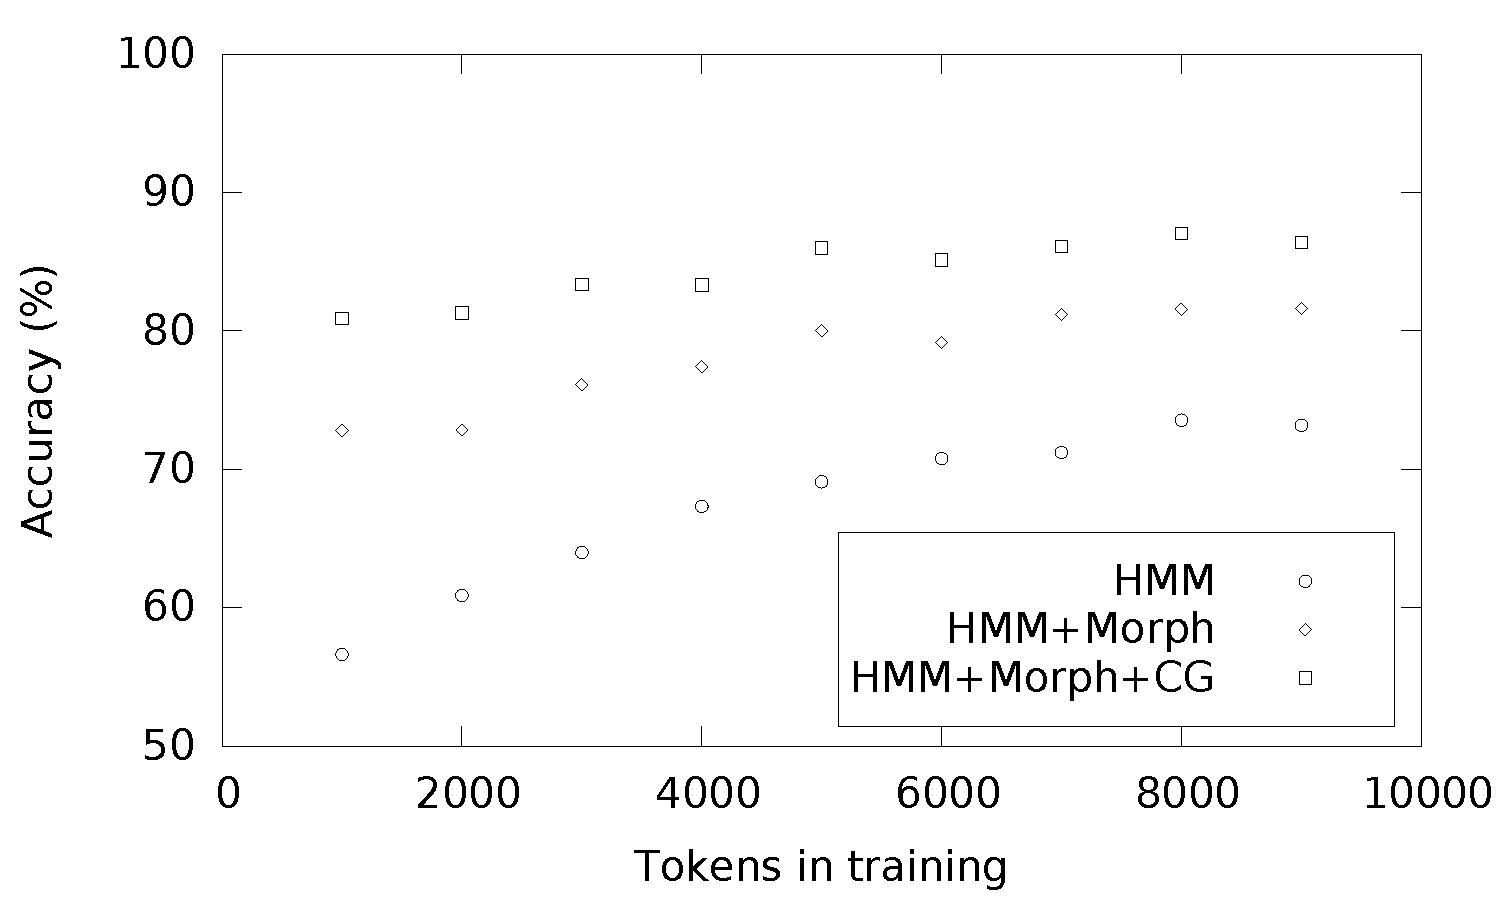
\includegraphics[width=0.70\textwidth]{graphics/learning-curve.pdf}
  \caption{Learning curve for three taggers, \texttt{hunpos} with no lexicon, 
    \texttt{hunpos} with a lexicon, and \texttt{hunpos} with a lexicon and the 
    Russian constraint grammar in a voting set up.}
  \label{fig:curve}
\end{figure*}

\section{Future work}
\label{sec:future}
% ROB
% FRAN
% func analysis
% dep analysis

% a CG+hmm could be much faster than tagging hundreds of thousands of words of text.

We have a number of plans for future work, the first of which is increasing the precision of the grammar without
decreasing recall. Secondly we would like to add syntactic function labelling and dependency parsing. For 
the dependency parser we plan to reuse the Giellatekno dependency grammar as in \cite{antonsen10}. 

The development workflow could also be improved, for example during the testing of each rule we could
save the correct decisions of the grammar. This would give us a partially-disambiguated development corpus,
which could be gradually used to build up a gold-standard corpus, and which could also be used for regression
testing to ensure that new rules added do not invalidate the correct decisions of previously written rules.

Also it is worth noting that although Russian has a great deal of non-free resources, this paper also presents
a method which is promising for smaller or lesser-resourced Slavic languages such as Sorbian, Rusyn or Belarusian. Instead
of hand-annotating a large quantity of text, it may be more efficient to work on grammatical resources --- such
as a morphological analyser and constraint grammar --- and use 
them alongside a smaller quantity of high-quality annotated text.

\section{Conclusions}
\label{sec:conclusions}

This paper has presented a preliminary constraint grammar for Russian, where rules have
been assigned to sections based on observations of performance on a non-gold corpus. The constraint grammar 
is high recall (over 0.99) and improves the performance over a trigram HMM-based tagger. It 
also shows state-of-the-art performance for the stress-placement task.

\section*{Acknowledgments}

We are grateful to Koen Claessen for insightful discussion, as well as three anonymous reviewers who 
gave thoughtful feedback on an earlier version of this paper. All remaining errors are our own. 

\bibliographystyle{acl}
\bibliography{ruscg}

\end{document}
